%************************************************
\chapter{Introduction}\label{ch:introduction}
%************************************************

\section{Compilers}
In order to understand what quantum circuit compilation is all about, it is helpful to first know what compilation means, and where our classical notions of compilation come from.
Merriam-Webster defines \textbf{compile} to mean % TODO how to cite this?
\begin{quote}
    to compose out of materials from other documents.
\end{quote}
We can see this definition reflected in~\citetitle{dragonbook}\footnote{Colloquially known as ``The Dragon Book'' because of the cover, and likely the most famous book on (classical) compilers.}\graffito{
    \centering
    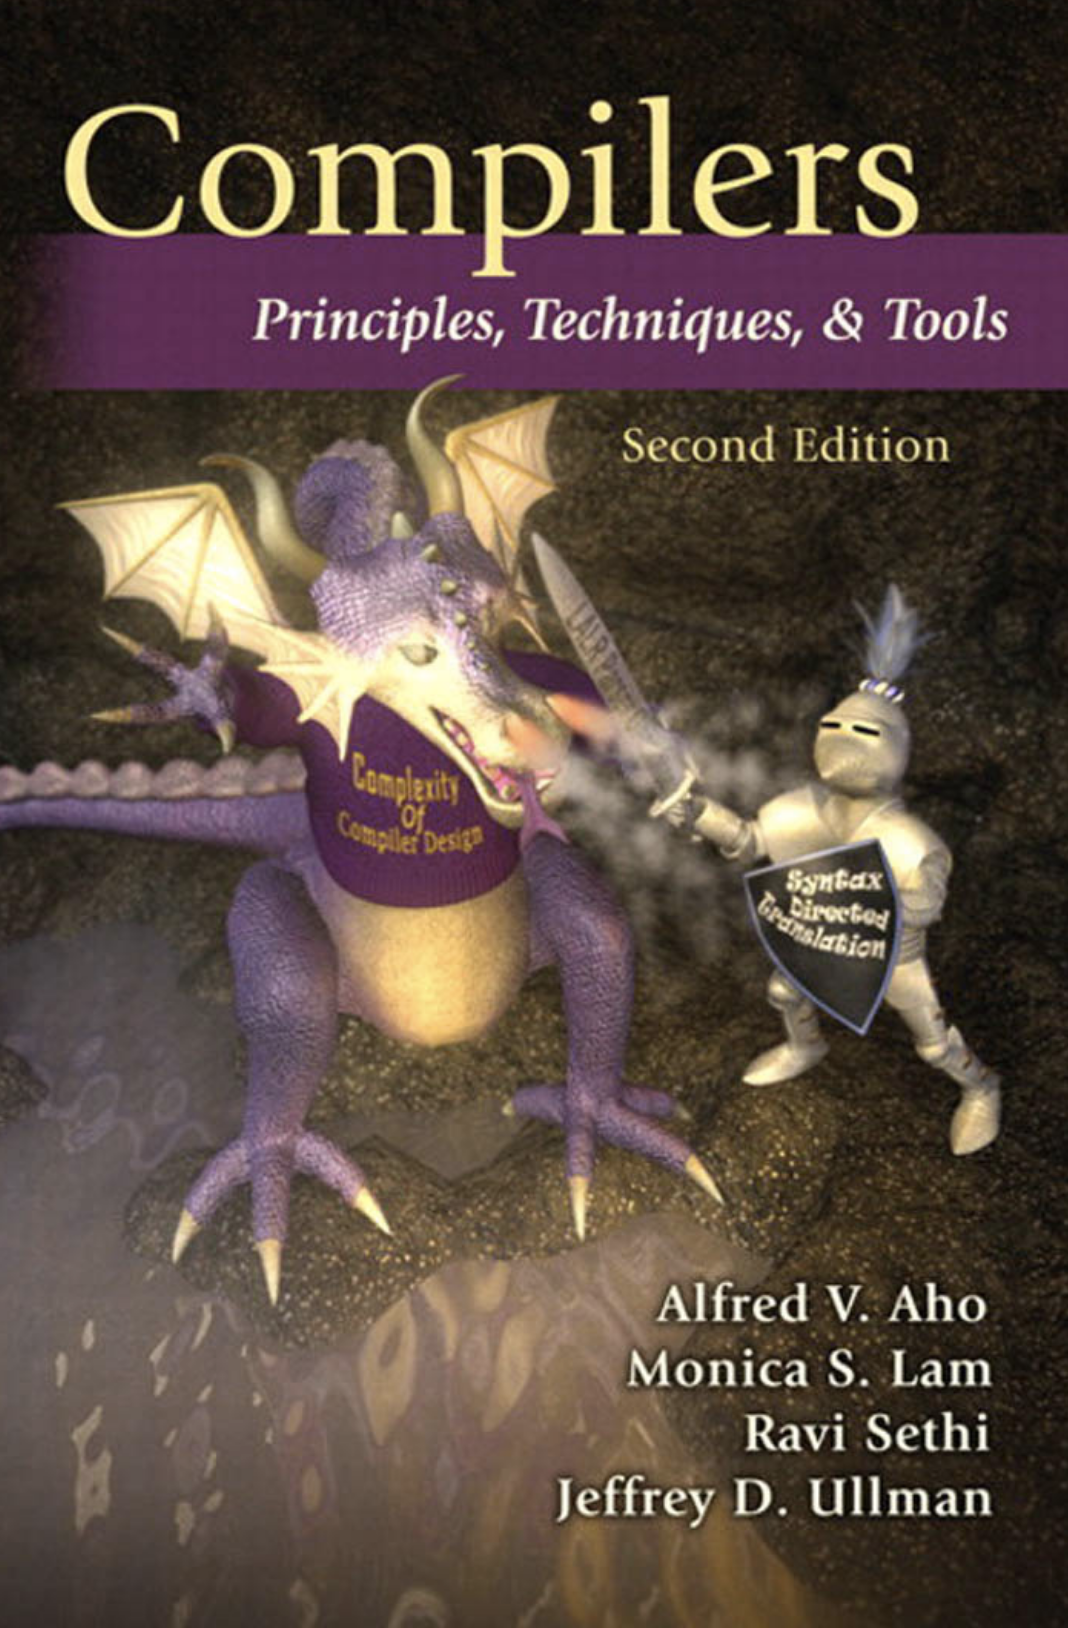
\includegraphics[width=\marginparwidth]{img/dragonbook.png}
    \emph{The Dragon Book}
}~\cite{dragonbook} where the authors introduce compilers through the process of transforming software.
\begin{quotation} % TODO technically the sentence doesn't start with Before, not sure how to formally quote it
    [B]efore a program can be run, it first must be translated into a form in which it can be executed by a computer.

    The software systems that do this translation are called \emph{compilers}.
\end{quotation}
Hence we can visualize the action of a compiler as a sort of informal function.
\begin{figure}[h]
    \centering
    \tikzset{
        frame/.style={
                draw,
                text width=6em,
                text centered,
                minimum height=4em,
                drop shadow,
                fill=orange!40,
                rounded corners,
            },
    }
    \begin{tikzpicture}[font=\sffamily, thick, node distance=4cm]
        \node[align=center] (pl) {Programming \\ Language};
        \node[frame, right of=pl] (compiler) {Compiler};
        \node[align=center, right of=compiler] (ml) {Machine \\ Language};

        \draw[-stealth] (pl) -- (compiler);
        \draw[-stealth] (compiler) -- (ml);
    \end{tikzpicture}
    \caption{Action of Compiler}
    \label{fig:compiler}
\end{figure}

The term compiler was coined by Grace Hopper in the early 1950's while working on a system that could translate symbolic mathematics into a machine language.
Initially Hopper was met with resistance for her new idea.
\begin{quotation}
    I had a running compiler, and nobody would touch it because, they carefully told me, computers could only do arithmetic; they could not do programs.
    It was a selling job to get people to try it.
    I think with any new idea, because people are allergic to change, you have to get out and sell the idea.
    \attrib{Grace Hopper 1952 \cite{hopperquote}}
\end{quotation}
In the end she succeeded in selling the idea and compilers became a ubiquitous piece of modern computing infrastructure.
Since Hopper coined the term the job of a compiler has grown enormously and now encompasses line reconstruction, preprocessing, lexical analysis, syntax analysis, semantic analysis, conversion to an \ac{IR}, optimization, target dependent optimizations, and finally code generation.
Thankfully we will not need to understand all of these parts, and the majority of this document will focus on \aclp{IR}, optimizations, and code generation.

\subsection{Examples of Compilers}
\begin{description}
    \item[\LaTeX{}:] While
    \item[Mathematica:]
    \item[Tensorflow:]
    \item[\texttt{clang}:]
\end{description}

\subsection{Computer Architecture}
To understand why it is we need compilers in the first place, we need to understand how modern computers work.
In a highly simplified model we can think of a computer as a \ac{CPU} connected to input and output devices (think keyboard and screen), and some sort of memory.
\begin{figure}[h]
    \centering
    \tikzset{
        frame/.style={
                draw,
                text width=6em,
                text centered,
                minimum height=4em,
                drop shadow,
                fill=orange!40,
                rounded corners,
            },
        line/.style={
                draw, -latex',rounded corners=3mm,
            }
    }
    \begin{tikzpicture}[font=\sffamily, thick, node distance=4cm]
        \node[frame](input){Input Device(s)};
        \node[frame, below=2cm](output){Output Device(s)};
        \node[frame, below right=-.15cm and 1cm of input](cpu){CPU};
        \node[frame, right of=cpu](memory){Memory};

        \path[line] (input) -| (cpu);
        \path[line] (cpu) |- (output);
        \draw[stealth-stealth] (cpu) -- (memory);
    \end{tikzpicture}
    \caption{A Simplified Computer Architecture}
    \label{fig:comparch}
\end{figure}

At the very basic level, a \ac{CPU} has a finite number of possible operations it can perform despite there being a much larger input space of ``possible programs'' that we can feed it.
How then does the computer take a script and run it on it's CPU?


Chris Lattner (the founder of one of the largest compiler projects; LLVM) has characterized compilers succinctly in~\cite{lattnerquote} as
\begin{quote}
    the art of allowing humans to think at a level of abstraction that they want to think about.
\end{quote}

\paragraph{Abstraction} With Lattner's quote in mind we can think of compilers as the tool that allows us to work with languages that are very abstract when compared to the instructions our \ac{CPU} can perform.
There also exist tools known as decompilers which take executables and turn them back into source code.
This operation is almost never the inverse of compiler because most languages allow for many ways of writing code that performs the same task.
With these tools we can raise and lower our levels of abstraction as desired and further push the details of the ``metal'' or hardware implementation away.


\section{LLVM}

% \subsection{\acf{MLIR}}